\documentclass[11pt, a4paper, twoside]{book}
\usepackage[utf8]{inputenc}
\usepackage[spanish]{babel}
%\usepackage{natbib}
\usepackage{apacite}
% Indice de palabras
\usepackage{makeidx}
\usepackage{acronym}

% ------- FIN usepackage -------------------------

% Here put the configuration of the document ------
% TODO: configuration of document
\usepackage{vmargin}
\setpapersize{A4}
\setmargins{2.5cm}		% margen izquierdo
{1.5cm}				% margen superior
{16.5cm}			% anchura del texto
{23.42cm}			% altura del texto
{10pt}				% altura de los encabezados
{1cm}				% espacio entre el texto y los encabezados
{0pt}				% altura del pie de página
{2cm}				% espacio entre el texto y el pie de página

% Interlineado
\renewcommand{\baselinestretch}{1.5}
% -------------------------------------------------
  
% Para que cree el indice de palabras
\makeindex % (pero aun no decimos donde)
% Tex con los acronimos
\chapter*{Lista de acrónimos}
\label{chap:acronimos}
\begin{acronym}[TESIS]
\acro{SW}{Software}
\acro{HW}{Hardware}
\acro{FT}{Tolerancia a Fallas}
\acro{FA}{Evitación de Fallas}
\acro{FR}{Eliminación de Fallas}
\acro{FF}{Predicción de Fallas}
\acro{MTBF}{Tiempo Medio Entre Fallas}
\acro{MTTF}{Tiempo Medio de Fallas}
\acro{MTTR}{Tiempo Medio de Reperación}
\acro{CMF}{Modo Común de fallas}
\acro{FDIR}{Detección, Aislación y Recuperación de Fallas}
\acro{CONAE}{Comisión Nacional de Actividades Espaciales}
\acro{UNLAM}{Universidad Nacional de La Matanza}
\acro{INVAP}{Investigación Aplicada}
\acro{NASA}{National Aeronautics and Space Administration}
\acro{COTS}{Commercial Off-The-Shelf}
\acro{TT}{Time-Trigged}
\end{acronym}


\makeatletter
\@addtoreset{chapter}{part}
\makeatother

\begin{document}
\frontmatter
\pagenumbering{Roman}
% Dedicatoria

\thispagestyle{empty}

\vspace*{4cm}
\hfill\normalsize\textit{\sf A mis padres}
\pagestyle{empty}

% Agradecimientos
\chapter*{Agradecimientos}
\label{chap:agradecimientos}
%\addcontentsline{toc}{chapter}{Agradecimientos}
En primer lugar, me gustaría agradecer a mi madre, que gracias a sus palabras de aliento, 
que me han acompañado en la distancia y a lo largo de estos dos años, hoy puedo estar
concretando esta meta. Sinceramente, si no fuese por ella, hoy estaría persiguiendo
otros objetivos. Desde chiquito me ha inculcado a que nunca debo bajar los brazos,
aún cuando todo parezca que está perdido. Siempre hay que luchar hasta el final.
Es por eso que hoy estoy aquí. Gracias mamá.

En segundo lugar, quiero agradecer a mi novia la Prof. Dra. Bioq. Brandán Yamila por su
comprensión, su compañía, su cariño, su amor y sus consejos. Además, quisiera agradecer y destacar
enormemente, que debido a su gran experiencia en el área de la investigación,
ha sabido guiarme y ayudarme en el desarrollo de esta tesis. Gracias amor. 

Por último lugar, quisiera agradecer a mis compañeros de maestría, Alfonso, Cecilia,
Eduardo, Elbio, Ezequiel, Javier, José, Pablo E., Pablo S. y Ricardo, por su amistad y
por compartir sus conocimientos. Gracias.




\pagestyle{empty}

% Resumen
\chapter*{Resumen} % si no queremos que añada la palabra "Capitulo"
%\addcontentsline{toc}{chapter}{Resumen} % si queremos que aparezca en el índice

Esta tesis se trata de
\pagestyle{empty}

% Indices
\cleardoublepage
\tableofcontents % indice de contenidos
\thispagestyle{empty}

\cleardoublepage
\addcontentsline{toc}{chapter}{Lista de figuras} % para que aparezca en el indice de contenidos
\listoffigures % indice de figuras

% Indice de palabra
\cleardoublepage
\addcontentsline{toc}{chapter}{Indice alfabético} % para que lo añada al índice de contenidos
\printindex % para que ponga el índice aquí



% Acronimos


\mainmatter	
%------------------------------------------------------------
% Introduccion
\pagenumbering{arabic}
\chapter{Introducción}\label{chap:intro}
% TODO: Introuducción, extraída desde el plan de tesis,
En el marco del Plan Espacial Nacional, desarrollado por la \ac{CONAE} de Argentina, y con el propósito de llevar a cabo actividades de investigación y 
aplicación, provenientes de la \ac{UNLAM} se presenta este plan de tesis con el fin de ampliar los 
conocimientos y la participación de la \ac{CONAE} y \ac{UNLAM}, en el campo del Desarrollo Informático y 
Ciencias de la Computación.

Las actividades desarrolladas para este trabajo de tesis son realizadas, en su mayor proporción, en 
la Unidad de Desarrollo \ac{INVAP}, ubicada en San Carlos de Bariloche, Provincia de Río Negro. Este 
trabajo se encuentra orientado a brindar un nuevo conocimiento, que ayude en cierta medida, en el 
desarrollo de los diferentes proyectos con los que cuenta actualmente esta empresa, agregando un 
grado de innovación en el resultado que se obtenga.

\ac{INVAP} tiene como visión ser un referente en proyectos tecnológicos a nivel mundial \cite{invapWEB}, 
por lo tanto, debe asegurarse que cada uno de los productos que se lleven a cabo sean competitivos. 
Para lograr cumplir con esto, es necesario que tales proyectos se encuentren a la vanguardia 
tecnológica y científica.  

El desarrollo de proyectos satelitales conlleva costos de importante magnitud, y 
dependen de cada misión. Una parte importante de los costos está conformado por el 
desarrollo\footnote{\textit{Nota: entiéndase por desarrollo al proceso de planificación, análisis, 
diseño e implementación.}} y sobre todo los materiales que se utilizan para su fabricación. Esto 
es debido a que se utilizan componentes que son exclusivos para el ámbito espacial, en otras 
palabras que se encuentran ``calificados para volar''. Estos componentes son fabricados especialmente para soportar el ambiente hostil del espacio.

Si se considera al ámbito espacial como una industria, algo que ha sido demostrado en los últimos 
años; y si se tiene en cuenta las intenciones de crecimiento y competitividad de la empresa INVAP,  de permitir el ingreso de nuestro pais en el mercado satelital \cite{invapWEB}, resulta de gran 
importancia lograr reducir los costos en fabricación y desarrollo de vehículos satelitales.

La \ac{NASA} tiene un enfoque de desarrollo bajo el lema 
``faster, cheaper, better'' \cite{Forsberg99}, lo cual busca desarrollar sus proyectos y misiones 
de foma rápida, barata y mejor. Bajo este enfoque se han realizado diversos estudios e 
investigaciones dando resultados sumamente positivos \cite{Tai99}, \cite{Chau99}, 
\cite{Schneidewind98}, \cite{Forsberg99}. En estos trabajos se utilizan componentes que no se 
encuentran ``calificados para volar'',  los cuales también son llamados componentes \ac{COTS}, o de estantería. Debe mencionarse, que también hubo algunos 
fracasos en su aplicación. 

A simple vista, la utilización de estos componentes ayudaría a reducir costos. Sin embargo, esto 
no es tan directo. Los componentes \ac{COTS} al no estar calificados, se les deben realizar tareas 
de calificación adicional. Además deben ser aplicados a un ambiente, que asegure 
que no fallarán durante la misión; o si fallan, no será motivo de pérdida de la misma. 

Los componentes \ac{COTS} suelen tener un costo de compra entre 100 y 1000 veces menores que aquellos 
que está califcados para volar. Por lo que el aumento en la utilización de estos componentes, 
aplicados al desarrollo de diferentes tipos de satélite, \textbf{permitiría reducir los costos y 
ahorrar algunos millones de dólares del proyecto satelital.} Esto facilitaría el ingreso de 
Argentina en un mercado altamente competitivo.

El desafío de este trabajo de tesis es analizar y estudiar arquitecturas que sean tolerantes a 
fallas, que permitan una correcta comunicación entre los diferentes subsistemas de un vehículo 
espacial de nueva generación, y que tenga como característica principal un cierto grado de confiabilidad, de modo tal que pueda ser aplicado con componentes \ac{COTS}.

\section{Motivación}\label{chap:motivacion}
Los costos de un proyecto satelital se pueden clasificar, a grandes rasgos, en 5 grupos:
\begin{itemize}
 \item Desarrollo
 \item Materiales
 \item Ensamblado, integración, y tests
 \item Lanzamiento
 \item Operaciones
\end{itemize}

Este trabajo de tesis se centrará principalmente en el desarrollo (proceso de planificación, 
análisis, diseño e implementación.), y en los materiales utilizados en la fabricación de vehículos satelitales.

No se puede mencionar a ciencia cierta cuál es el costo “verdadero” de desarrollar un satélite. Este 
depende exclusivamente del tipo de satélite y de la misión. Lo que si se debe tener en claro es que 
las tareas de desarrollo representan una parte muy importante del costo total del proyecto.

Desarrollar un vehículo espacial con componente \ac{COTS}, en un principio podría representar costos 
adicionales, ya que se le deben realizar tareas de calificación adicional, debido a que no están 
“preparados” para resistir las condiciones hostiles del espacio. 

Uno de los puntos positivos, y que motivan la aplicación de componentes COTS, es que a la hora de 
desarrollar varios satélites en base a la misma ingeniería, se puede ahorrar en gran medida en los 
materiales que se utilizan. Los componentes \ac{COTS} suelen tener un costo de compra entre 100 y 1000 
veces menores que aquellos que están calificados para volar. \textbf{Esto ayudaría a ahorrar 
algunos millones de dólares de los proyectos satelitales.}
  
Otra de las ventajas de utilizar componentes \ac{COTS}, es que la mayoría cuentan con una tecnología más 
avanzada que aquellos que son calificados para volar. Esta tecnología permite:
\begin{itemize}
 \item Aumentar prestaciones, mediante el incremento de las capacidades de procesamiento, memoria, 
velocidades de 
procesamiento, etc.
 \item Implementar funciones que son imposibles de aplicar en tecnologías viejas.
 \item Reducir tiempos de desarrollo.
 \item Reducir volumen, masa y consumo
\end{itemize}

El último punto mencionado anteriormente es de especial interés, ya que al reducir volumen y masa, 
permite reducir costos adicionales como el de lanzamiento.

Esta reducción de costos de proyectos satelitales tienen ventajas directas a la hora de introducir a 
Argentina en un mercado altamente competitivo, donde la mínima reducción de estos, representa 
ganancias económicas importantes. 
 
Uno de los puntos en contra de la utilización de componentes \ac{COTS} es que al no ser calificados para 
volar, es necesario llevar a cabo tareas y estrategias inteligentes, con el fin de hacer frente a 
esa “deficiencia”. Por ello, se exige realizar una investigación y análisis de diferentes 
arquitecturas de aviónica, que puedan ser utilizadas para lograr que el sistema sea tolerante a 
fallas, y así, cumplir con los requerimientos de una misión satelital. 

El estudio de arquitecturas tolerantes a fallas, no solamente tiene aplicación en el ámbito 
espacial, si no que también puede ser extendido a cualquier sistema crítico, los cuales necesitan 
ser robustos y tolerantes a fallas, como es el caso de aviones comerciales, plantas nucleares, 
automóviles, etc.

% --------------------- %
% TODO: Hipótesis
% --------------------- %
\section{Hipótesis}
La hipótesis de esta tesis es la siguiente: ``Una arquitectura de aviónica  basadas en componentes 
\ac{COTS}, robusta y tolerante a fallas, es totalmente aplicable y utilizable en vehículos espaciales, 
con un alto nivel de confiabilidad, lo cual permite disminuir la complejidad de los sistemas actuales de aviónica''.

\section{Objetivo del trabajo y preguntas de investigación}

\subsection{Objetivo}
El objetivo de este trabajo es investigar y analizar arquitecturas de comunicación de los 
subsistemas de aviónica tolerante a fallas basada en componentes \ac{COTS} para vehículos 
satelitales de nueva generación.

% secondary objectives
\subsection{Objetivos Específicos}
\begin{enumerate}
 \item Realizar un estudio del estado de la cuestión sobre arquitecturas tolerantes a fallas para 
sistemas críticos.
 \item Investigar y analizar arquitecturas tolerantes a fallas que aseguren la confiabilidad del 
sistema y que sean aplicables en la industria satelital.
 \item Investigar y analizar protocolos de comunicación, para las capas superiores del modelo de 
OSI (modelo de interconexión de sistemas abiertos - ISO/IEC 7498-1), orientados a la tolerancia a 
fallas y confiabilidad de los sistemas. Realizar un estudio comparativo de los diferentes 
protocolos estudiados.
 \item Investigar una metodología para lograr una medición de la tolerancia a fallas en 
arquitecturas de aviónica.
 \item Desarrollar un estudio comparativo de arquitecturas tolerantes a fallas con el fin de obtener 
ventajas y desventajas de cada una de ellas.
 \item Diseñar modelos alternativos de arquitecturas tolerantes a fallas, que tenga un grado de 
confiabilidad tal que permita la aplicación de componentes \ac{COTS}.
 \item Evaluar la confiabilidad de los modelos de arquitecturas (mediante métrica desarrollada en 
este trabajo o siguiendo otras estrategias). 
 \item Proponer el diseño de una nueva arquitectura tolerante a fallas, con un 
grado de confiabilidad suficiente para la aplicación de componentes \ac{COTS} en aviónicas de vehículos 
satelitales.
\item Simular la arquitectura planteada para medir su grado de tolerancia a fallas y perfomance.
\end{enumerate}


% Tolerancia a fallas
%\chapter{Software tolerante a fallas}
\section{Tolerancia a falla}\label{chap:FaultTolerance}
En sistemas críticos, como el de una planta nuclear, sistemas médicos, el sistema de vuelo 
de un avión, o el de un satélite, tanto \ac{SW} (como el hardware) no deben fallar, ya que esto daría 
como resultado la pérdida de vidas humanas, como así también perdidas de dinero.
Para el caso particular, del vehículo espacial 
(satélite, transbordador, lanzador), la falla del \ac{SW} podría tener como consecuencia el
fracaso de una misión, y/o una gran cantidad de dinero, y hasta vidas humanas en algunos caso (como pueden ser en vuelos 
tripulados). La principal diferencia entre el \ac{SW} de una misión satelital, con la de un avión 
o una planta nuclear, o un sistéma médico, es que ante alguna falla o error, se torna complicado 
llegar hasta el satélite para realizar una actualización o cargar un parche de \ac{SW}.

La \cite{IEEE610.12} define como \ac{SW} crítico a ``aquel cuyo fracaso puede tener un impacto en 
la seguridad, o puede causar grandes pérdidas financieras o sociales''. El \ac{SW} de estos 
sistemas críticos deben tener la capacidad de seguir funcionando, aún en la presencia de fallas, o 
errores. Imaginese el caso, de un avión comercial, con pasajeros a bordo, y de repente ocurre un 
problema debido al mal diseño del \ac{SW} (por ejemplo un overflow de memoria). En esta situación 
es impensable que el \ac{SW} se congele y que el piloto reinicie el sistema, esperar que se 
reestablezca al estado en el cual se encontraba antes del problema, para seguir funcionando. Lo 
mismo ocurre con el \ac{SW} de naves espaciales, hay situaciones en la que no se puede esperar y es 
preferible que el sistema siga funcionando aún en la presencia de fallas.

Tal como lo indica \cite{pressman01} las fallas de \ac{SW} implican problemas cualitativos que son 
descubiertos después de que el \ac{SW} es llevado a los usuarios y probados por ellos. Una 
gran cantidad de estudios indican que en las actividades de diseño se introducen entre un 50 y 65 
porciento de errores del total de errores que se dan durante el proceso del \ac{SW} 
\citep{pressman01}. Esto no debe ocurrir en el ámbito espacial, ya que una vez que el sistema es 
utilizado, es muy difícil corregir los errores que surgen 

Cabe aclarar que el \ac{SW} al no ser un componente físico, no puede ser tratado de la misma 
manera que un componenete hardware. Como ejemplifica \cite{SoftwareFaultToleranceATutorial}, las 
fallas que surgen a nivel de bit, como por ejemplo en un disco duro, son fallas del dispositivo de 
almacenamiento y pueden ser mitigadas con la aplicación de técnicas de redundancias. Esto no es así 
para el \ac{SW}. Por lo tanto evitar los errores a nivel de \ac{SW} no es tan trivial como 
en el hardware.

A nivel de \ac{SW} las fallas son llamadas ``bugs'' (tal como se indica en la
sección~\ref{sec:terminologia} en la página~\pageref{sec:terminologia}), y existe 
un solo tipo de fallas que es introducido durante el desarrollo del \ac{SW} 
\citep{SoftwareFaultToleranceATutorial}. Las fallas en el \ac{SW} son el principal motivo de que 
todo un sistema fracase. 

La \ac{FT}, puede ser utilizada como una capa más de protección 
\citep{SoftwareFaultToleranceATutorial}. Esta aplicada al \ac{SW} se refiere al uso de técnicas que 
permiten seguir brindando el servicio en un nivel aceptable de perfomance y seguridad después que 
una falla de diseño ocurra. 

Debe hacerse una diferencia entre \ac{FT} y calidad. \cite{Hanmer07} lo define de la 
siguiente manera: ``\ac{FT} es la capacidad del sistema a ejecutarse apropiadamente a 
pesar de la presencia de fallas. \ac{FT} ocurre en tiempo de ejecución''. Cuando se 
habla que un sistema es tolerante a fallas, significa que fue diseñado de tal manera, que 
puede seguir funcionando correctamente aún en la presencia de errores de sistemas \citep{Hanmer07}. 

En cambio calidad, tal como lo define \cite{Hanmer07}, ``se refiere a cuán libre de fallas está el 
sistema. Técnicas de calidad que indican cómo el \ac{SW} es creado. Si el sistema fue testeado.'' 

Un sistema de alta calidad tendrá menor número de fallas, que esto representa menor número de 
fallas en tiempo de ejecución. La reducción del número de fallas no implica que los resultados de 
los defectos son menos severos \citep{Hanmer07}. El sistema debe tomar medidas para reducir el 
impacto de los errores y fallas, y es allí donde surge la \ac{FT}.	

Un sistema tolerante a fallas provee una continua y segura operación, aún durante la presencia 
de fallas. Un sistema tolerante a fallas, es un elemento crítico para una arquitectura de vuelo, lo 
cual incluye hardware, \ac{SW}, timing, sensores y sus interfaces, actuadores, elementos y datos 
de comunicación con los diferenes elementos \citep{FTAvionics}. 

Este tipo de sistemas debería detectar los errores causados por fallas, evaluar los daños 
producidos por la falla, aislar a la misma y por último recuperarse, en ese caso se habla de 
aquitectura o sistemas \acs{FDIR}\footnote{FDIR, del inglés: Failure detect, isolate and recover}.

\ac{FT} es la capacidad de un sistema a continuar funcionando a pesar de la ocurrencia 
de fallas \citep{FTDesign}. Un sistema tolerante a fallas debe ser capaz de manejar fallas tanto de 
hardware como de \ac{SW}. La \ac{FT} es necesaria debido a que es imposible construir 
un sistema perfecto.

El objetivo de la \ac{FT} es el desarrollo de sistemas que tengan la capacidad de
funcionar correctamente en 
presencia de fallas \citep{FTDesign}. La \ac{FT} es alcanzada mediante la utilización de redundancias \citep{FTDesign}. \textit{Redundancia} es la provisión de capacidades 
funcionales que sería innecesario para entornos libres de fallas \citep{FTDesign}. Esto significa 
tener hardware adicionales, check bits en una cadena de datos, o algunas l\'ineas de c\'odigo que 
verifique el resultado correcto del \ac{SW}. La redundancia permite enmascarar una falla, o 
detectarla, para luego localizarla, contenerla y recuperarse de esta \citep{FTDesign}. Las 
técnicas de tolerancia de fallas se emplean durante la adquisición, o desarrollo del \ac{SW}. 
Permite al \ac{SW} tolerar fallas después que este haya sido desarrollado \citep{Pullum01}. Cuando 
una falla se da, las técnicas de \ac{FT} proveen mecanismos al sistema de \ac{SW} para prevenir el 
fracaso del sistema \citep{Pullum01}.

%\section{Clasificación de un sistema de control tolerante a fallas}

\section{Redundancia en el software}\label{sec:redundancias_sw}
A pesar de lo comentado anteriormente, sobre la importancia del \ac{SW}, todavía existe una 
creencia, de que el \ac{SW} aparece por arte de magia, y que los programadores no son nunca, lo 
suficientemente capaces, de hacer un \ac{SW} libre de errores. Salvo aquellas empresas u 
organizaciones que tienen un proceso maduro de desarrollo de \ac{SW}, el resto suele encasillarse
en el pensamiento mencionado anteriomente. 

\cite{FTDesign} explica que la \ac{FT} aplicado en el \ac{SW} no está tan entendido, ni maduro, 
como es en el caso de la \ac{FT} aplicada en hardware. Si una falla exisitiera en el \ac{SW}, esta 
se haría ``visible'', solo cuando las condiciones relevantes ocurran \citep{FTDesign}. Y muchas 
veces por tiempo o costo, no se realizan los tests cubriendo todos los posibles ambientes reales, 
lo cual tiene consecuencias desastrosas, tal como se expone en la sección~\ref{chap:motivacion} 
(página~\pageref{chap:motivacion}).

Para sistemas complejos o grandes, donde existe una gran cantidad de estados, implica que solo una 
pequeña porción del \ac{SW} puede ser verifcada correctamente \citep{FTDesign}. Los tests 
tradicionales y métodos de depuración actuales no alcanzan para grandes sistemas \citep{FTDesign}. 
La utilización de métodos formales para describir las característica requeridas por el 
comportamiento del \ac{SW} exigen gran complejidad computacional, y solo son aplicables en 
ciertas situaciones \citep{FTDesign}.

Las técnicas de \ac{FT} se pueden dividir en dos grupos:
\begin{itemize}
 \item técnicas de una sola versión (single version), se utilizan cuando existe una sola versión del \ac{SW} en el 
sistema.
 \item técnicas multi-versión (multi-version), se utilizan cuando se desarrollan varias versiones de una misma 
función. 
\end{itemize}

Estas se explican en las siguientes secciones.

\subsection{Técnicas single version}
Estas técnicas son utilizadas para tolerar parcialmente las fallas del diseño de \ac{SW} 
\citep{Pullum01}. Técnicas single-version de \ac{FT} se basa en el uso de redundancia aplicada a 
una única versión de una pieza de \ac{SW} para detectar y recuperarse de fallas 
\citep{SoftwareFaultToleranceATutorial}. 

Estas técnicas le brindan a los software que cuentan con una sola versión, un número de capacidades funcionales 
que no serían necesarias dentro de un ambiente libre de fallas \citep{FTDesign}. 

\subsubsection{Estructuras de software}
En \cite{SoftwareFaultToleranceATutorial} se mencionan dos técnicas de estructuración del \ac{SW}
que presentan características favorables al momento de mantener \ac{FT} en el \ac{SW}.

La definición de una arquitectura en el software es de suma importancia ya que proveen las bases para 
la implementación de \ac{FT} \citep{SoftwareFaultToleranceATutorial}. Una de las técnicas utilizadas 
en el desarollo del software es la modularización. Esta consiste en descomponer el problema en 
componentes manejables. Esto tiene como resultado que sea más eficiente la aplicación de la \ac{FT} 
en el diseño de un sistema \citep{SoftwareFaultToleranceATutorial}. 

El particionado es otra técnica mencionada en \cite{SoftwareFaultToleranceATutorial}, lo cual 
provee aislación entre módulos independentes del sistema. Esta técnica permite descomponer al 
problema en partes separadas \citep{pressman01}. El particionado puede ser horizontal u 
vertical. En el primero se descompone el problema moviéndose en forma horizontal en la jerarquía, 
mientras que el segundo se parte de lo más general hasta llegar a lo detallado, moviendose 
verticalmente en la jerarquía \citep{pressman01}. 

Sistema de cierre es un principio de \ac{FT}, en el cual ninguna acción es permitible sin una 
autorización expresa \citep{SoftwareFaultToleranceATutorial}. Siguiendo este principio ninguna de 
las funciones que componen al sistema deberían tener más capacidad de la necesaria 
\citep{SoftwareFaultToleranceATutorial}. Las ventajas de desarrollar un sistema bajo este principio, 
es que es sencillo el manejo de errores, y evitar la propagación de fallas si ocurriesen. 

\subsection{Técnicas multi-version}
Las técnicas de multi-version utilizan dos o más versiones diferentes del mismo módulo de \ac{SW} 
(\citep{FTDesign}; \citep{SoftwareFaultToleranceATutorial}), lo cual satisface el requerimiento de 
diversidad. 

El objetivo de utilizar diferentes versiones de \ac{SW} es que es construido de diferentes 
maneras, por lo tanto fallarían de diferente maneras \citep{SoftwareFaultToleranceATutorial}.

\subsection{Técnicas de detección de fallas}
Para los \ac{SW} tolerantes a fallas de una sola versión, se suelen utilizar varios tests de 
``aceptación'' para detectar fallas \citep{FTDesign}. Es necesario que estos \ac{SW} cuenten con 
dos propiedades: auto protección\footnote{En inglés, self-protection} y auto check\footnote{En 
inglés, self-checking} \citep{SoftwareFaultToleranceATutorial}. La auto protección significa que  
los componentes del sistema tienen la capacidad de protegerse así mismo mediante la detección de 
errores \citep{SoftwareFaultToleranceATutorial}. La propiedad de auto check significa que los 
componente son capaces de detectar fallas internas y tomar las acciones necesarias para evitar la 
propagación del error. 

El resultado del sistema depende del resultado de los tests. Si el resultado pasa exitosamente el 
test, este es el correcto, caso contrario significa la presencia de fallas \citep{FTDesign}. Un test 
es más efectivo si se puede calcular de una manera simple \citep{FTDesign}. 

Las técnicas utilizadas son las siguientes:
\begin{itemize}
 \item \textit{Timing checks:} se agrega a los sistemas una restricción de tiempo. Basado en esa 
restricción se puede deducir si el comportamiento del sistema se desvió \citep{FTDesign}. Los más 
utilizado es el \textit{watchdog timer}, este es un contador que se actualiza con un \textit{timer} que 
detecta si un módulo de \ac{SW} se bloqueó o congeló, entonces se reinicia ese módulo o el sistema. 
 \item \textit{Coding checks:} se utiliza en los sistemas donde los datos se codifican usando 
técnicas de redundancia de datos \citep{FTDesign}. 
 \item \textit{Reversal checks:} son aquellos donde se toma los valores de salida, y con ellos se 
busca encontrar cuáles fueron los datos de entrada. Si los datos de entrada reales coinciden con 
los calculados (para una misma salida), este se encuentra libre de fallas \citep{FTDesign}. 
 \item \textit{Reasonableness checks:} usa propiedades semánticas en los datos para detectar 
fallas \citep{FTDesign}. 
 \item \textit{Structural checks:} se basa en el conocimiento de las propiedades de la estructura 
de datos \citep{FTDesign}. 
 \item \textit{Replication checks: } se basa en la comparación de resultados de varios componentes 
\citep{SoftwareFaultToleranceATutorial}. 
\end{itemize}

Se suelen utilizar árboles de fallas, como una técnica auxiliar en el desarrollo de sistemas para 
la detección de fallas \citep{SoftwareFaultToleranceATutorial}. El árbol de falla permite obtener 
un enfoque top-down de las diferentes fallas que se pueden dar. El árbol no cubre todas las fallas 
que puedan darse, pero si ayudan en un alto grado en el desarrollo de \ac{SW} tolerante a fallas 
\citep{SoftwareFaultToleranceATutorial}. 

\subsection{Técnicas de recuperación de fallas}
Una vez que la falla es detectada, el sistema debe proceder a recuperarse de aquella, y volver a 
un estado operacional normal \citep{FTDesign}. Si los mecanismos de deteccíón y contención de 
fallas fueron desarrollados correctamente, esta es contenida dentro de un set de módulos en el 
momento de la detección \citep{FTDesign}. 

\subsubsection{Manejo de excepciones}
En muchos \ac{SW} y lenguajes de programación, los errores se pueden recuperar mediante el manejo de 
excepciones. El manejo de excepciones es la interrupción del funcionamiento normal para responder a 
un funcionamiento anormal del sistema \citep{SoftwareFaultToleranceATutorial}. Los posibles eventos 
que pueden lanzar una excepción son:
\begin{enumerate}
 \item Excepciones de interfaces, son lanzadas por un módulo cuando se da una solicitud inválida de 
algún servicio \citep{FTDesign}.
 \item Excepciones locales, son lanzadas por algún módulo cuando sus propios mecanismos de 
detección de fallas encuentran un problema interno \citep{FTDesign}.
 \item Excepciones de fracaso, son lanzadas cuando un mecanismos de detección encuentra una falla, 
pero es imposible recuperarse de esa falta \citep{FTDesign}.
\end{enumerate}

\subsubsection{Checkpoint y Restart}
Para los software de una sola versión existen pocos mecanismos de recuperación. Checkpoint y restart 
es uno de ellos. También es conocido como \textit{backward error recovery} \citep{FTDesign}. La 
mayoría de las fallas que se dan en los \ac{SW} son debido a fallas que provienen del diseño, tal 
como se mencionó anteriomente. Estas fallas son activadas por entradas al sistema \citep{FTDesign}. 

Este mecanismo cuenta con el módulo principal que se encuentra en ejecución combinado con un bloque 
que realiza tests de aceptación. Si se detecta una falla, en el bloque de testeo, se envía una 
señal de ``reincio'', para que el módulo principal vuelva al estado anterior, es decir, antes de 
producirse el error. Este estado anterior se encuentra almacenado en una memoria checkpoint 
\citep{FTDesign}. En la figura \ref{fig:checkAndRestart}\footnote{Basado en \cite{FTDesign} y 
\cite{SoftwareFaultToleranceATutorial}}, se muestra la representación de este mecanismo.

\begin{comment}
\begin{figure}[h]
  \centering
  \begin{tikzpicture}
  % definicion de estilos
  \tikzstyle{cuadro} = [draw, sep=5,rectangle,minimum height=3em, minimum width=6em, node 
  distance=2cm] 

  \tikzstyle{vacio} = [inner, sep=5,rectangle,minimum height=3em, minimum width=6em, node 
  distance=3cm] 

  \tikzstyle{circulo} = [fill, shape=circle, minimum size=5pt, inner sep=3pt, node distance=4cm ]
  
  % cuadros
  \node[cuadro] (checkMemo){Memoria de Checkpoint};
  \node[cuadro , below of=checkMemo, pin={[->] left:Entrada}] (modulo){Módulo en ejecución};
  \node[circulo, right of=modulo] (circ){};
  \node[cuadro, below of=circ] (detector){Test de aceptación};
  \node[vacio, right of = circ] (salida){Salida};

  \draw[->] (checkMemo.-30)--(modulo.30);
  \draw[->] (modulo.150) -- (checkMemo.-150);
  \draw[->] (modulo)--(circ);
  \draw[->] (circ)--(salida);
  \draw[->] (circ)--(detector);
  \draw[->] (detector)-|(modulo) node[near end, left] {retry};
  \end{tikzpicture}
  \caption{Representación de checkpoint y restart}
  \label{fig:checkAndRestart}
\end{figure}
\end{comment}

\begin{figure}[h]
 \centering
 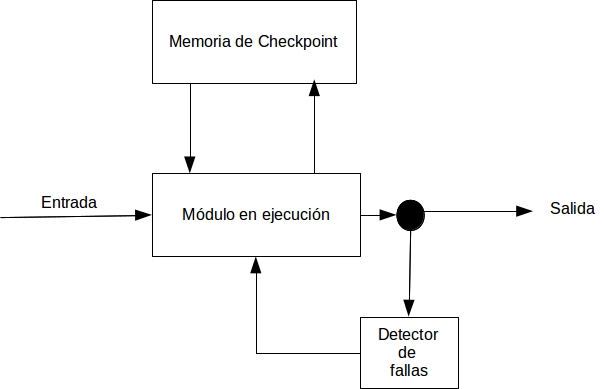
\includegraphics[scale=0.5]{images/Marco_teorico/checkAndRestart.jpg}
 \caption{Representación de checkpoint y restart}
 \label{fig:checkAndRestart}
\end{figure} 


Existe dos tipos de checkpoints, estáticos y dinámicos. Los checkpoints estáticos toman una 
``fotografía'' del estado del sistema antes de comenzar la ejecución del \ac{SW} y lo guarda en la
memoria \citep{FTDesign}. Si se detecta una falla, el sistema regresa a ese estado y 
comienza de nuevo su ejecución \citep{FTDesign}. Los checkpoints estáticos se basan en regresar el 
módulo a un estado predeterminado \citep{SoftwareFaultToleranceATutorial}. Se puede regresar a un 
estado inicial o a un set de estados predeterminados \citep{SoftwareFaultToleranceATutorial}.

Por otro lado se encuentran los checkpoints dinámicos. Estos usan checkpoints creados 
dinámicamente. Estas son imágenes del estado del sistema en varios puntos durante la ejecución 
\citep{SoftwareFaultToleranceATutorial}.

Hay tres formas de crear los checkpoints dinámicamente:
\begin{enumerate}
 \item Equidistantes, en el cual los intervalos que se crean los checkpoints son siempre iguales, 
los intervalos se elijen teniendo en cuenta el rate de falla \citep{FTDesign}. 
 \item Modular, en el cual los checkpoints se crean al principio o al final de la ejecución de un 
módulo. 
 \item Random, los checkpoints se crean aleatoriamente en el tiempo. 
\end{enumerate}

\subsubsection{Procesos pares}
Los procesos a pares utilizan dos versiones idénticas de un proceso de \ac{SW} que corre en 
procesadores separados (\citep{FTDesign}; \citep{SoftwareFaultToleranceATutorial}). El mecanismo de 
recuperación que se utiliza es el de checkpoint y restart \citep{SoftwareFaultToleranceATutorial}.  

Como se puede observar en la figura~\ref{fig:repPares}\footnote{Basada en \cite{FTDesign} y 
\cite{SoftwareFaultToleranceATutorial}} el primer procesador se encuentra activo. Este envía un 
checkpoint al segundo procesador. Si una falla se detecta, el primer procesador se apaga y se cambia 
al segundo procesador. El segundo procesador carga el checkpoint y continua con la operación.Toma el 
rol del primer procesador \citep{SoftwareFaultToleranceATutorial}. Luego el 
primer procesador realiza un auto test para verificar si el problema continua. Si se encuentra que 
este procesador sigue teniendo problema, se continúa trabajando con el segundo procesador 
\citep{FTDesign}.

La principal ventaja que brinda este mecanismo según \cite{FTDesign} es que permite entregar el 
servicio ininterrumpidamente.

\begin{figure}[h]
 \centering
 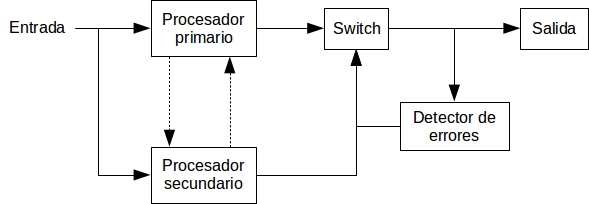
\includegraphics[scale=0.6]{images/Marco_teorico/repPares.jpg}
 \caption{Representación del proceso pares}
 \label{fig:repPares}
\end{figure} 

\begin{comment}

\begin{figure}[h]
 \centering
 \begin{tikzpicture}[node distance=1cm, auto,]
  % definicion de estilos
  %Define style for boxes
   \tikzset{
   cuadro/.style={
           rectangle,
           draw=black,
           text width=6.5em,
           minimum height=2em,
           text centered},
    % Define arrow style
    arrow/.style={
           ->,
           thick,
           shorten <=2pt,
           shorten >=2pt,}	
    }
  \tikzstyle{circulo} = [draw, fill=black, circle, node distance=1cm, minimum size=5pt, inner 
sep=3pt]
    
  % Gráfico
  \node[inner sep=5pt] (entrada) {Entrada};
  \node[cuadro, right=0.5cm of entrada] (prim) {Procesador Primario};
  \node[cuadro, inner sep=5pt,below=0.5cm of prim] (secu) {Procesador Secundario};
  \node[cuadro, inner sep=10pt, right=1cm of prim] (selec) {Switch};
  \node[inner sep=0pt, right=2cm of selec](ghost1){};
  \node[cuadro, below=0.5cm of ghost1](detector) {Detector de error};
  \node[inner sep=0pt, right=0.5cm of ghost1] (salida) {Salida};
  
  \draw[arrow] (entrada)--(prim);
  \draw[arrow] (entrada)|-(secu);
  \draw[arrow, dashed] (prim.-30) -- (secu.30);
  \draw[arrow, dashed] (secu.150) -- (prim.-150);
  \draw[arrow] (prim)--(selec);
  \draw[arrow] (secu)-|(selec.-150);
  \draw[arrow] (detector)-|(selec);
  \draw[arrow] (selec)--(salida);
  \draw[arrow] (ghost1)--(detector);
 \end{tikzpicture}
 \caption{Representación del proceso pares}
 \label{fig:repPares}
\end{figure}

\end{comment}

\subsubsection{Diversidad de datos}
La diversidad es una técnica utilizada para mejorar la eficiencia en los checkpoint y restart, 
usando diferentes entradas por cada reinicio. Esto se basa en que las fallas en el 
\ac{SW} son dependientes de las entradas. Es poco probable que la misma falla se 
de con la misma secuencia de entrada \citep{FTDesign}.

\subsubsection{Bloques de recuperación}

Esta técnica combina las bases de la técnica de checkpoints y restart enfocada con múltiples 
versiones de un componente de \ac{SW} en el sentido de que una versión de \ac{SW} diferente es 
lanzada cada vez que se encuentra una falla. Los 
checkpoints son creados antes de que una versión de \ac{SW} se ejecuta.
La ejecución de las múltiples versiones pueden ser 
secuencial o paralelas dependiendo de la disponibilidad de la capacidad de procesamiento y 
perfomance requerida \citep{SoftwareFaultToleranceATutorial}.

%La representación de esta técnica se puede observar en el figura~[AGREGAR IMAGEN].
Las 
versiones son diferentes implementaciones de un mismo programa. Solo una de estas versiones provee 
la salida del sistema. Si un error es detectado por el test de aceptación, se vuelve hacia atrás, 
se retoma el último checkpoint, y se vuelve a ejecutar el módulo de \ac{SW} pero con una 
versión diferente a la que se ejecutó anteriormente \citep{FTDesign}.  	

Los checks del test de aceptación deben mantenerse simples para mantener la velocidad de la 
ejecución \citep{FTDesign}.

\begin{comment}
\begin{figure}[h]
 \centering
 \begin{tikzpicture}[node distance=1cm, auto,]
  % definicion de estilos
  %Define style for boxes
   \tikzset{
   cuadro/.style={
           rectangle,
           draw=black,
           text width=6.5em,
           minimum height=2em,
           text centered},
    % Define arrow style
    arrow/.style={
           ->,
           thick,
           shorten <=2pt,
           shorten >=2pt,}	
    }
       
  \tikzstyle{circulo} = [draw, fill=black, circle, node distance=1cm, minimum size=5pt, inner 
sep=3pt]
    
  % Gráfico
  \node[inner, sep=5pt] (input1){Entrada 1};
  \node[inner, sep=5pt, below=0.5cm of input1] (input2){Entrada 2};
  \node[inner, sep=5pt, below=0.5cm of input2] (puntos1){...};
  \node[inner, sep=5pt, below=0.5cm of puntos1] (inputn){Entrada n};
  \node[cuadro, right=0.5cm of input1] (version1){Versión 1};
  \node[cuadro, right=0.5cm of input2] (version2){Versión 2};
  \node[inner, sep=5pt, right=2cm of puntos1](puntos2){...};
  \node[cuadro, right=0.5cm of inputn] (versionn){Version n};
  
  \node[cuadro, above=1cm of version1] (check) {Memoria Checkpoint};
  \node[cuadro, right=1cm of version2] (switch) {Swith n a 1};
  \node[inner, sep=0pt, right=1cm of switch](ghost1){};
  \node[cuadro, below=0.5cm of ghost1](test){Test de aceptación};
  
  \node[inner, sep=0pt, right=0.5cm of ghost1](output){Salida};
 
  %Arrows
  \draw[arrow] (input1)--(version1);
  \draw[arrow] (input2)--(version2);
  \draw[arrow] (inputn)--(versionn);
  \draw[arrow] (version1)-|(switch.west);
  \draw[arrow] (version2)--(switch);
  \draw[arrow] (versionn)-|(switch.west);
  \draw[arrow] (ghost1)--(test);
  \draw[arrow] (switch)--(output);
  
  \draw[arrow, dashed] (check.-40) -- (version1.30);
  \draw[arrow, dashed] (version1.150) -- (check.-145);
  
  

 \end{tikzpicture}
 \caption{Configuración de bloques de recuperación}
 \label{fig:repPares}
\end{figure}
\end{comment}

%\subsubsection{Programación N-version}

%\subsubsection{Programación N-Auto Checking}



% ----------------------------------------------------------------------------------------------
\backmatter
\newpage
\nocite{*}
\bibliography{../Bibliography/biblio}
%\bibliographystyle{apalike}
\bibliographystyle{apacite}
\addcontentsline{toc}{chapter}{Bibliograf\'ia}

\end{document}
  
  